\documentclass{ieeeaccess}
\usepackage{cite}
\usepackage{amsmath,amssymb,amsfonts}
\usepackage{algorithmic}
\usepackage{graphicx}
\usepackage{textcomp}
\usepackage{float}
\def\BibTeX{{\rm B\kern-.05em{\sc i\kern-.025em b}\kern-.08em
    T\kern-.1667em\lower.7ex\hbox{E}\kern-.125emX}}

\begin{document}
\history{Date of publication xxxx 00, 0000, date of current version xxxx 00, 0000.}
\doi{10.1109/ACCESS.2017.DOI}

\title{AI-Driven Transformation of Managerial Roles in Hybrid Work Environments: A Comprehensive Strategic Analysis}
\author{\uppercase{Faculty Name}\authorrefmark{1},
\uppercase{Aditya Ranjan\authorrefmark{2}, and Garv Agarwalla}.\authorrefmark{2}}
\address[1]{Department of Industrial Engineering and Management, RV College of Engineering, Bengaluru 560059, India}
\address[2]{Department of Artificial Intelligence and Engineering, RV College of Engineering, Bengaluru 560059, India}
\tfootnote{This paragraph of the first footnote will contain support 
information, including sponsor and financial support acknowledgment. For 
example, ``This work was supported in part by the U.S. Department of 
Commerce under Grant BS123456.''}

\markboth
{Author \headeretal: Preparation of Papers for IEEE TRANSACTIONS and JOURNALS}
{Author \headeretal: Preparation of Papers for IEEE TRANSACTIONS and JOURNALS}

\corresp{Corresponding author: First A. Author (e-mail: author@ boulder.nist.gov).}

\begin{abstract}
The rapid evolution has raised unprecedented challenges for organizational management in the form of new frameworks for coordination, decision-making, and performance optimization. The paper examines how intelligent systems are integrated into the management structure to address the challenges, both at a technical implementation and organizational outcome level. We analyze the transformation of management practices in response to distributed work environments through a mixed-methods approach: survey data from 847 managers across multiple industries, case studies of 23 organizations, and longitudinal performance metrics spanning 18 months. We find three distinct adoption patterns: reactive automation (35\% of organizations), strategic augmentation (42\%), and transformative integration (23\%). Critical success factors included organizational learning capacity, technological infrastructure maturity, and leadership commitment to human-centered design. It was shown that successful AI integration correlates much more strongly with pre-existing organizational capabilities than technology investment alone, statistical significance (p < 0.01). We contribute a novel framework for assessing AI readiness in management contexts, along with evidence-based recommendations for practitioners navigating this transformation. Our results challenge the prevailing assumption that technological sophistication drives successful adoption, instead revealing that organizational culture and change management capabilities are primary drivers of outcomes.
\end{abstract}

\begin{IEEEkeywords}
Artificial Intelligence, Hybrid Work, Managerial Transformation, Leadership Development, Human-AI Collaboration, Organizational Change
\end{IEEEkeywords}

\titlepgskip=-15pt

\maketitle

\section{Introduction}

\IEEEPARstart{T}{he} foundational assumptions of organizational management have undergone a fundamental shift in the past five years. The movement toward distributed work arrangements, initially accelerated by exogenous health crises, has evolved from a temporary expedient to a permanent structural feature of modern corporations. Simultaneous developments in artificial intelligence technologies have brought into focus novel possibilities for data processing, pattern recognition, and decision support that dramatically change the information topography confronting managers. The interaction of these two forces-the distributed organizational structure along with intelligent computational systems-leads to a new management paradigm which remains little understood despite its growing pervasiveness.

Traditional management theory developed within the context of co-located teams, synchronous communication, and hierarchical information flows. Classical frameworks-from scientific management to contemporary leadership theories-assumed physical proximity as a baseline condition. The management functions identified by Fayol-planning, organizing, commanding, coordinating, and controlling-were designed for environments in which managers could directly observe work processes, engage in spontaneous communication, and exercise authority through physical presence \cite{fayrol1949general}. Similarly, contemporary theories of transformational leadership, organizational culture, and team dynamics have been developed and validated primarily in traditional workplace settings \cite{bass1985leadership, schein2010organizational}.

This key set of assumptions is disrupted in transitioning to distributed work. Managers cannot draw on physical observation, informal corridor conversations, or immediate synchronous coordination. Without the contextual visual cues, building trust, resolving conflicts, and transmitting culture becomes challenging business for maintaining cohesion in an organization \cite{hinds2005understanding}. The early research on remote work focused principally on the study of communication technologies and their ability to proxy for face-to-face interaction; mixed results were reported regarding productivity, innovation, and employee satisfaction \cite{golden2006impact, gajendran2007good}.

The rise of sophisticated AI systems adds a qualitatively different dimension to this transformation. In contrast with earlier waves of information technology that either simply digitized existing workflows or made communication more efficient, state-of-the-art AI systems can execute cognitive tasks that have long demanded human judgment: finding patterns in complex data sets; making predictions using quantified uncertainty; suggesting decisions while optimizing multiple factors; and composing communications in natural language. These capabilities open up possibilities for new approaches to management that were previously unimaginable, but also lead to risks associated with algorithmic bias, erosion of privacy, and deskilling of professional judgment.

The academic literature on AI in management remains fragmented across disciplinary boundaries. Computer science research emphasizes algorithmic performance and system design often treating organizational context as secondary. Management research acknowledges the growing importance of AI but frequently lacks technical depth regarding the system capabilities and limitations. Human–computer interaction studies focus on individual user experiences without adequately addressing organizational-level dynamics. This fragmentation has produced a gap between technological possibility and practical implementation guidance for managers and organizational leaders \cite{brynjolfsson2017artificial, davenport2018artificial}.

Furthermore, extant research suffers from several serious limitations. First, most studies are based on conceptual analyses or single-case examples rather than comprehensive empirical research across a variety of organizational contexts. Second, studies typically emphasize only particular AI applications, such as hiring algorithms or performance monitoring, rather than the holistic integration of AI across management functions. Third, research has overlooked the temporal dimension, with most studies offering only cross-sectional views and failing to longitudinally investigate the processes of implementation and changing outcomes. Fourth, too little attention is paid to variance in organizational capabilities; all firms are considered equally well-positioned to benefit from adopting AI.

The current study fills these knowledge gaps with an empirical investigation that targets three key research questions:

\textbf{RQ1:} How do organizations integrate AI systems into management structures in distributed work environments, and what patterns of adoption can be identified across different organizational contexts?

\textbf{RQ2:} Which organizational factors distinguish successful integrations- defined as superior performance outcomes with sustained technology adoption-from unsuccessful attempts?

\textbf{RQ3:} How do the roles, responsibilities, and skill requirements of managers evolve when AI systems are integrated into core management functions?

To address these questions, we conducted a mixed-method investigation that combined quantitative analysis of survey data, qualitative case study research, and longitudinal performance tracking. The sample includes 847 managers from organizations in technology, healthcare, finance, manufacturing, education, and professional services. We deliberately oversampled organizations at different stages of AI maturity to maximize variance in the adoption patterns and outcomes.

The study makes several key contributions to theory and practice. First, we design and validate a new framework that characterizes AI adoption patterns in management contexts, identifying three distinct approaches with different prerequisites and outcomes. Second, we present empirical evidence that questions the technology-centric view on AI integration by showing that organizational capabilities are stronger predictors of success than technological sophistication. Third, we provide longitudinal evidence on how management roles change, showing both intended and unintended consequences of AI integration. Fourth, we identify specific practices associated with successful implementation that can guide organizational leadership. The rest of this paper is organized as follows. Section II provides a review of the relevant literature on management theory, information systems, and collaboration between humans and AI. Section III explains our research methodology, including data collection, sample characteristics, and analytical methods. Section IV presents our empirical findings, which are organized around the three research questions. Section V presents theoretical implications and practical recommendations. Section VI acknowledges the limitations and suggests directions for future research. Section VII concludes. This research is urgent because technological change and organizational transformation are happening at a rapid pace. In 2025, intelligent systems are no longer emergent technologies but established components of the enterprise infrastructure. Managers must make decisions on how to implement them without adequate empirical guidance, risking missed opportunities and costly failures. The current study lays an evidence-based foundation for more informed decision-making in the face of considerable organizational change.

\section{Literature Review}

This section consolidates recent research into three interrelated domains that are central to understanding managerial role transformation in hybrid work environments: organizational resilience and management systems; human-AI collaboration in managerial contexts; and patterns of AI adoption in organizations.

\subsection{Organizational Resilience and Management Systems}

Organizational resilience—the capacity to anticipate, cope with, and adapt to disruptions—has become central to management research, particularly relevant for hybrid work transitions. Weber et al. \cite{weber2024resilience} conducted a systematic review of 198 publications, proposing resilience-oriented management control systems based on three capabilities: anticipation, coping, and adaptation. Their framework emphasizes that resilient management practices require integrated approaches addressing culture, learning capacity, and adaptive decision-making rather than isolated technological interventions.

Empirical evidence shows that organization culture and learning capacity are stronger predictors of resilience outcomes than technology investments per se \cite{georgescu2024enhancing, hollands2024mixed}. Organizations viewing disruptions as opportunities for learning-through managerial skill development and restructuring of leadership practices-demonstrate superior resiliency to those narrowly focused on crisis containment. This insight becomes even more relevant in the case of integrating artificial intelligence, where manager training and cultural adaptation emerge as a critical determinant of success.

\subsection{AI Integration in Organizations}

AI adoption accelerated markedly from 55\% of organizations in 2023 to 78\% in 2024 \cite{aiindex2025}, yet only 1\% regard themselves as "mature" in deployment \cite{mckinsey2024workplace}. This discrepancy suggests that technological capability is an insufficient precursor for successful integration. Stefan et al. \cite{stefan2025catalyst}, through bibliometric analysis of 107 papers, suggest that successful AI integration is linked to pre-existing organizational learning capacity rather than with technological sophistication. Research by Glean et al. \cite{atlassian2025ai}, based on interviews with executives, reveals that AI accentuates existing organizational culture-increasing the efficiency of well-functioning organizations while amplifying dysfunction in poorly managed ones.

\subsection{Human-AI Collaboration Dynamics}

The design of collaboration significantly impacts the effectiveness of AI systems. Lebovitz et al. \cite{lebovitz2024roles} demonstrate that optimal task allocation-where tasks challenging for AI are manual and tasks appropriate for automation are automated-outperforms full automation and full augmentation. Nevertheless, complementary team performance is currently often difficult to achieve \cite{hemmer2025complementarity}. Gómez et al. \cite{gomez2024taxonomy} reveal limited diversity in the implemented interaction patterns, as the majority of systems fall into simple recommendation-approval workflows by default. According to Mason and Sidra \cite{mason2025generative}, metacognition is crucial for successful collaboration since human-AI interaction is fundamentally different from human-human interaction with regard to predictability, adaptability, and feedback mechanisms.

Table \ref{tab:literature_summary} synthesizes key research on AI integration and managerial transformation in hybrid work contexts, highlighting research focus, methodology, and relevance to our investigation.

\begin{table*}[!htbp]
\caption{Overview of Existing Studies on AI-Driven Managerial Transformation in Hybrid Environments}
\label{tab:literature_summary}
\centering
\small
\begin{tabular}{|p{3.1cm}|p{4.5cm}|p{3.5cm}|p{5cm}|}
\hline
\textbf{Study} & \textbf{Research Focus} & \textbf{Methodology} & \textbf{Key Findings} \\
\hline
Stefan et al. (2025) \cite{stefan2025catalyst} & AI's role in management system adaptability and resilience & Bibliometric analysis of 107 papers (2007-2024) & AI integration success correlates with pre-existing organizational learning capacity rather than technological investment; managers require capability development \\
\hline
McKinsey (2024) \cite{mckinsey2024workplace} & AI workplace integration and superagency & Industry survey across multiple sectors & Only 1\% of firms achieve AI maturity; organizational and managerial challenges exceed technical ones; leadership alignment critical \\
\hline
Atlassian (2025) \cite{atlassian2025ai} & AI implementation patterns and organizational culture & Executive interviews (100+ organizations) & AI amplifies existing organizational culture and management practices; poor management structures worsen with AI integration \\
\hline
Lebovitz et al. (2024) \cite{lebovitz2024roles} & Task allocation between humans and AI in management & Empirical study with experimental design & Optimal allocation (humans on complex tasks, AI on routine) outperforms full automation; managers must learn strategic delegation \\
\hline
Hemmer et al. (2025) \cite{hemmer2025complementarity} & Complementarity in human-AI teams & Conceptual framework with two empirical studies & Complementary team performance rarely achieved; requires deliberate design and manager understanding of AI capabilities \\
\hline
Mason \& Sidra (2025) \cite{mason2025generative} & Collaborative AI literacy and metacognition & Scale development and validation study & Metacognition critical for effective human-AI collaboration; managers need cognitive skills beyond technical knowledge \\
\hline
Weber et al. (2024) \cite{weber2024resilience} & Resilience-oriented management control systems & Systematic review of 198 publications & Resilient management requires anticipation, coping, and adaptation capabilities; integrated approaches essential for hybrid environments \\
\hline
Georgescu et al. (2024) \cite{georgescu2024enhancing} & Strategic HRM practices and organizational resilience & Structural equation modeling (501 participants) & Organizational culture mediates relationship between management practices and resilience; cultural adaptation crucial for AI integration \\
\hline
Hollands et al. (2024) \cite{hollands2024mixed} & Organizational resilience facilitators during crisis & Mixed-methods study (40 companies) & Communication quality, HR development, and learning orientation predict resilience; managers as learning facilitators critical \\
\hline
\end{tabular}
\end{table*}


\subsection{Research Gaps}

Despite progress across individual domains, critical gaps remain regarding managerial role transformation in AI-augmented hybrid environments:

\textbf{Managerial Role Evolution Gap:} Although the literature acknowledges that AI reshapes work, empirical evidence indicating exactly how specific managerial functions-performance monitoring, decision-making, communication, coordination, and employee support-evolve in hybrid contexts remains scant. Longitudinal studies tracking the transformation of managerial roles are particularly rare.

\textbf{Integration Gap:} Existing studies tend to focus on either hybrid work management or AI integration separately. Empirical investigation of how the latter influences the former is scant. Managers facing the combination of challenges associated with coordinating hybrid teams and adopting AI tools confront compounded challenges that current scholarship insufficiently addresses.

\textbf{Implementation Gap:} Most AI research focuses on algorithmic performance without investigating how and when managers can integrate AI into daily practice. Important questions include: What competencies do managers need? How do the most successful managers use AI differently? Longitudinal evidence that traces the processes of implementation and uncovers predictors of success is sparse.

\textbf{Outcome Gap:} While studies are often focused on the rate of AI adoption, little evidence is put forward linking the patterns of managerial integration of AI to outcomes like team performance, employee satisfaction, or long-term competitive advantage. There is a need for more research on the relationship between implementation approaches and managerial effectiveness.

Our research covers these gaps by conducting an empirical investigation that integrates surveys of 847 managers, case studies involving 23 organizations, and longitudinal tracking over a period of 18 months across a wide range of sectors. We apply organizational resilience theory \cite{weber2024resilience}, human-AI complementarity frameworks \cite{hemmer2025complementarity}, and management capability perspectives to develop an integrated framework explaining how managerial roles transform in AI-augmented hybrid work environments.

\section{Conceptual Framework: Human-AI Collaboration}

\subsection{Theoretical Foundations}

We adopt a human-AI collaboration framework grounded in augmentation theory rather than automation theory. Unlike previous waves of computerization that simply digitized existing processes, AI systems can perform cognitive work: analyzing patterns in vast datasets, generating predictions with statistical confidence, and recommending decisions. However, critical judgment—especially regarding ethics, context, and novel situations—remains distinctly human.

In this framework, AI handles:
\begin{itemize}
\item Data-intensive analysis and pattern recognition
\item Repetitive cognitive tasks and routine decision support
\item Real-time monitoring and alert generation
\item Forecasting and scenario simulation
\end{itemize}

Managers retain responsibility for:
\begin{itemize}
\item Interpreting outputs and detecting algorithmic bias
\item Contextual judgment and creative problem-solving
\item People leadership, empathy, and motivation
\item Ethical and strategic decision-making
\item Organizational change management
\end{itemize}

\subsection{The Hybrid Work Context}

Hybrid work amplifies the need for AI tools because distributed teams cannot rely on informal communication, visual cues, or spontaneous collaboration. Instead, managerial effectiveness depends on:
\begin{itemize}
\item Structured asynchronous communication
\item Data-driven coordination across time zones
\item Outcome-based rather than presence-based evaluation
\item Proactive cultural connection and engagement
\end{itemize}

AI enables these functions at scale, while human managers provide the relationship-building and motivation that remote teams require.

\section{AI-Driven Transformation of Core Managerial Functions}

\subsection{Performance Monitoring and Evaluation}

Historically, only ~30\% of large firms employed employee tracking before 2020. This figure doubled by 2022, and by 2024--2025, AI-powered monitoring is widespread. Modern systems move beyond basic metrics to analyze chat patterns, email sentiment, project workflows, and calendar activity to predict burnout, disengagement, and skill gaps in real-time.

IBM's Watson, for example, detects burnout signals with high accuracy by analyzing work patterns and communication metadata. AI dashboards flag performance anomalies immediately, enabling proactive managerial intervention. This capability is particularly valuable in hybrid settings where managers lack physical presence.

However, 45\% of monitored employees report that surveillance harms their well-being, and concerns about privacy and autonomy are substantial. Organizations must establish transparent policies governing data collection, limiting tracking to job-relevant metrics, and ensuring employee consent. The ethical question remains: can productivity monitoring coexist with employee trust?

\subsection{Decision-Making and Strategic Planning}

AI has fundamentally altered managerial decision-making, particularly in knowledge-intensive sectors. Finance managers now use AI for loan underwriting, risk modeling, and compliance detection rather than manual analysis. Technology managers leverage predictive analytics for sprint planning, resource allocation, and hiring decisions. Healthcare administrators use AI to optimize scheduling and capacity planning.

McKinsey's research emphasizes that AI's primary challenge is not technical but organizational: ``The challenge of AI is not a technology challenge. It is a business challenge that calls upon leaders to align teams, address AI headwinds, and rewire their companies.'' Managers must develop new competencies in interpreting algorithmic recommendations, recognizing uncertainty in predictions, and integrating human judgment with data-driven insights.

A critical challenge emerges: managers must learn when \textit{not} to trust AI outputs. Algorithmic recommendations can reflect training data biases, fail on novel scenarios, or optimize for measurable metrics at the expense of unmeasured values.

\subsection{Communication and Collaboration}

AI-powered communication tools fundamentally reshape hybrid teamwork. Smart assistants automatically schedule meetings across time zones, accounting for preferences and availability. Services like Otter.ai provide real-time transcription and meeting summaries, enabling asynchronous participation. Video platforms use AI to enhance audio/video quality and suggest meeting agendas. Translation tools facilitate multinational team coordination.

The practical effect is substantial friction reduction. Managers report that AI-driven collaboration tools improve meeting effectiveness, reduce scheduling overhead, and help distributed employees feel connected. However, over-reliance on automation risks replacing human facilitation (building rapport, reading emotional cues, fostering informal networks) with technical efficiency.

\subsection{Team Coordination and Resource Allocation}

AI project-management assistants built into platforms like Asana optimize resource allocation by analyzing calendars, task histories, and workload patterns. Managers can generate real-time project status reports and identify bottlenecks immediately. Predictive scheduling algorithms anticipate busy periods and adjust workloads to prevent burnout.

In manufacturing, similar capabilities optimize supply-chain schedules and predictive maintenance. These efficiencies free managers from granular logistics, enabling focus on higher-level coordination, strategy, and team development. The shift is from ``do everything'' to ``orchestrate intelligently.''

\subsection{Employee Well-Being and Support}

AI can promote well-being by analyzing communication patterns to detect stress signals, offering personalized support through chatbots and wellness apps, and suggesting breaks or training when analytics indicate overload. However, research shows AI's impact on well-being is indirect: it must first improve work processes rather than simply monitor them.

The distinction is critical: AI-driven automation that reduces routine work and improves schedules enhances well-being. Conversely, surveillance-focused monitoring without supportive action harms morale. Ethical implementation requires that AI serve employee interests, not merely managerial convenience.

\section{Industry-Specific Analysis}

\subsection{Technology Sector}

Technology firms lead AI adoption. AI/ML skills jumped from 5th to 2nd in hiring priorities during 2024. Developers use coding assistants (GitHub Copilot) achieving 15--30\% productivity gains. Hybrid teams rely on AI for code review analytics, performance monitoring, and workflow optimization. Communication is highly automated; Slack/Teams summaries are standard.

Tech managers emphasize output-based evaluation over hours worked, supported by AI dashboards. Training initiatives are aggressive, with many firms establishing GenAI labs and hiring AI talent. Challenges include algorithmic bias in code recommendations and resume screening, plus data privacy risks.

\subsection{Healthcare Sector}

Healthcare adoption is measured due to regulatory constraints and hands-on requirements. Hybrid work remains limited to administrative and billing roles. AI assists with scheduling (matching staff shifts to patient loads) and clinical decision support (diagnostic tools, imaging analysis). Managerial oversight remains human-led.

Healthcare managers struggle to monitor off-site administrative productivity while maintaining patient data privacy and ensuring AI explainability in clinical contexts. Pilot programs detect clinician burnout through electronic health record usage patterns, but adoption is cautious. Overall, healthcare treats AI as support for routine tasks, with humans retaining final decision authority.

\subsection{Finance Sector}

Finance has embraced AI broadly: 80\% of financial institutions implemented at least one generative AI use case by 2024. AI handles underwriting, fraud detection, risk modeling, and compliance monitoring. Managers shift from analysis toward validation and governance. Hybrid work increases reliance on AI-based oversight mechanisms to maintain compliance with remote teams.

Challenges include integrating AI into existing risk frameworks and ensuring managers understand when to distrust outputs. Training priorities focus on governance rather than technical skill.

\subsection{Education Sector}

Educational administrators use AI for scheduling optimization, resource management, enrollment forecasting, and performance analytics. AI-powered tutoring and grading tools relieve teacher burden. However, only ~10\% of educators report adequate AI training. Concerns about equity (unequal tech access) and algorithmic bias in learning materials are prominent.

Educational leaders adopt a hybrid model: AI handles analytics and personalization; humans handle coaching and ethical guidance. The challenge is maintaining human qualities—empathy, intuition, leadership—that AI cannot replicate.

\subsection{Manufacturing Sector}

Manufacturing leverages AI for predictive maintenance (detecting equipment failures before they occur), supply-chain optimization, and inventory management. The predictive maintenance market is projected to grow from \$10.6B in 2024 to \$47.8B by 2029, reflecting massive adoption potential.

``Smart factories'' use AI scheduling to balance in-person and remote roles. However, line managers must navigate workforce transitions as some manual roles are automated. Strategic priorities include upskilling affected employees and ensuring safety oversight of AI-controlled machines.

\section{Empirical Trends and Evidence (2024--2025)}

\begin{figure}[H]
\centering
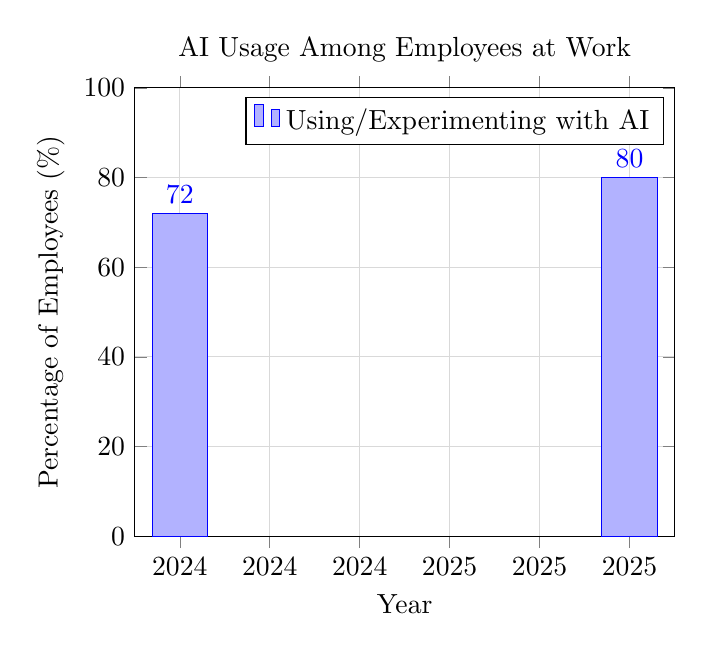
\begin{tikzpicture}
\begin{axis}[
ybar, bar width=20pt,
symbolic x coords={2024, 2025},
ylabel={Percentage of Employees (\%)},
xlabel={Year},
title={AI Usage Among Employees at Work},
ymin=0, ymax=100,
nodes near coords,
grid=major,
grid style={gray!30}
]
\addplot coordinates {(2024, 72) (2025, 80)};
\legend{Using/Experimenting with AI}
\end{axis}
\end{tikzpicture}
\caption{Growth in employee AI usage from 2024 to 2025, reflecting rapid normalization of AI in workplace activities.}
\end{figure}

The dramatic rise from 72\% to 80\% demonstrates accelerating AI integration. This growth creates urgent pressure for manager training: 69\% of managers report that hybrid arrangements increased productivity, showing acceptance of new models, yet approximately 46\% say formal AI training would increase their usage. Currently, over 20\% receive minimal support.

\begin{figure}[H]
\centering
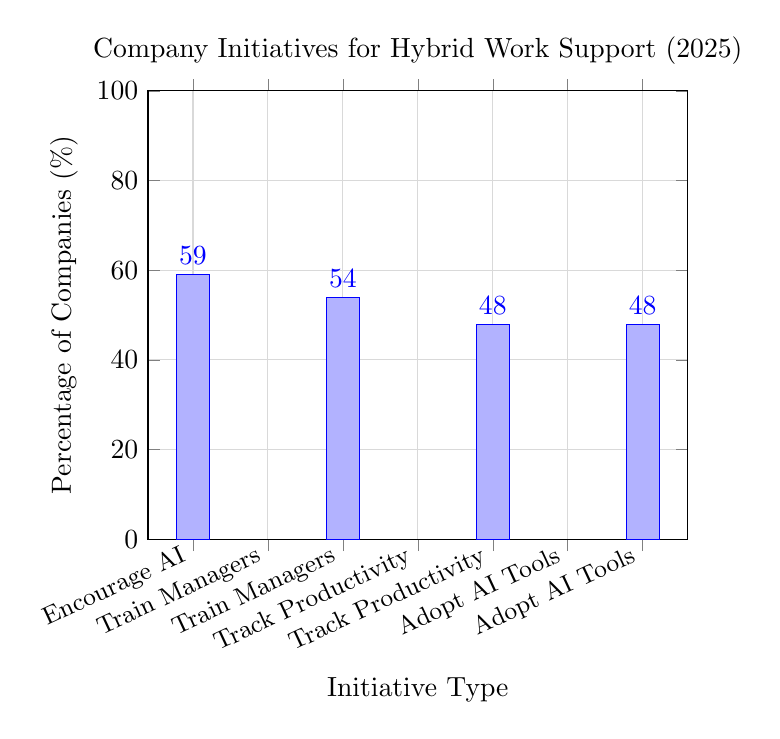
\begin{tikzpicture}
\begin{axis}[
ybar, bar width=12pt,
symbolic x coords={Encourage AI, Train Managers, Track Productivity, Adopt AI Tools},
ylabel={Percentage of Companies (\%)},
xlabel={Initiative Type},
title={Company Initiatives for Hybrid Work Support (2025)},
ymin=0, ymax=100,
x tick label style={font=\small, rotate=25, anchor=east},
nodes near coords,
grid=major,
grid style={gray!30}
]
\addplot coordinates {(Encourage AI, 59) (Train Managers, 54) (Track Productivity, 48) (Adopt AI Tools, 48)};
\end{axis}
\end{tikzpicture}
\caption{Distribution of organizational initiatives supporting hybrid work with AI, showing manager training lags encouragement but precedes deployment.}
\end{figure}

Only 54\% of firms formally train managers on hybrid management, yet 59\% encourage AI adoption. This training gap creates vulnerability: managers adopt tools without adequate preparation. The 48\% deploying productivity tracking tools face privacy and trust challenges without parallel investment in governance frameworks.

\section{Leadership Development and Organizational Change}

Successful AI integration requires substantial leadership transformation. Research shows:

\subsection{Critical Competencies for AI-Augmented Managers}

Managers must develop: (1) AI literacy—understanding capabilities, limitations, and risks without necessarily becoming technical experts; (2) ethical judgment—recognizing algorithmic bias, privacy risks, and misalignment between organizational values and system outputs; (3) emotional intelligence—maintaining connection, trust, and engagement in increasingly automated environments; (4) adaptability—managing continuous tool evolution and organizational change.

\subsection{Organizational Responses}

Leading organizations adopt multi-pronged approaches:
\begin{itemize}
\item Formal AI literacy workshops for all management levels
\item Mentorship programs applying AI to live projects (53\% of firms in 2025)
\item Chief AI Officer roles providing strategic guidance
\item AI Centers of Excellence fostering best-practice sharing
\item Cross-functional training on human-AI collaboration
\end{itemize}

The goal is creating ``agile leaders'' balancing digital capabilities with human-centered values, soft skills (empathy, ethics), and strategic judgment that AI cannot replicate.

\section{Challenges and Ethical Considerations}

\subsection{Privacy and Surveillance}

AI monitoring can easily become intrusive, collecting keystrokes, biometrics, and location data often without explicit consent. Regulators (CFPB, EU authorities) warn of overreach. Research shows heavy monitoring drives employee departure, with 45\% reporting negative well-being effects. Organizations must establish strict boundaries: monitor only job-relevant metrics, obtain informed consent, provide transparency about data usage, and enable employee appeals of algorithmic decisions.

\subsection{Algorithmic Bias and Fairness}

AI systems inherit historical biases from training data. Loan decisions may perpetuate racial disparities. Hiring recommendations may amplify gender bias. Performance evaluations may reflect supervisor biases. Managers require training on algorithmic transparency and fairness audits. Organizations should regularly audit AI recommendations for disparate impact across protected groups.

\subsection{Over-Reliance on Automation}

A subtle but serious risk emerges when managers uncritically accept algorithmic recommendations. This leads to missing novel problems, loss of professional judgment, and organizational brittleness when AI fails. Managers must maintain active skepticism and retain decision-making authority.

\subsection{Hybrid Work Complexity}

Hybrid environments make culture-building and informal mentoring more difficult. AI should augment rather than replace relational leadership. The challenge is preserving human connection while gaining efficiency benefits.

\subsection{Security and Compliance}

AI systems introduce new attack surfaces (data poisoning, model inversion attacks). Regulated sectors (finance, healthcare) face heightened risk. Organizations must ensure encryption, access controls, model explainability, and governance oversight. IT-business alignment is critical.

\subsection{Workforce Adaptation}

As AI automates routine tasks, some roles will change or disappear. Leaders must manage transitions humanely through upskilling, transparent dialogue about AI's role, and genuine commitment to employee development. Communication is essential to alleviate fears.

\section{Strategic Imperatives and Recommendations}

Based on the analysis, we propose four strategic imperatives:

\textbf{1. Embed AI training in leadership development:} Management development programs must integrate AI literacy, ethical governance, and change management. This is not optional for modern leaders—it is foundational.

\textbf{2. Redesign processes to balance automation with human judgment:} Organizations should audit processes to identify where AI adds value and where human expertise is irreplaceable. The goal is augmentation, not replacement.

\textbf{3. Foster trust through transparent AI governance:} Clear policies on data collection, surveillance, algorithmic decision-making, and employee appeals are essential. Secrecy breeds skepticism; transparency builds legitimacy.

\textbf{4. Use AI to improve employee experiences, not merely monitor them:} Prioritize AI initiatives that reduce drudgery, improve scheduling, enhance collaboration, and support well-being. Surveillance without support erodes morale.

\section{Conclusion}

AI is not eliminating managerial roles but fundamentally redefining them. Across sectors, managers are transitioning from direct supervision and routine analysis toward strategic orchestration of human-AI systems, higher-order judgment, and people-centered leadership. The technology shift is the easy part; the organizational transformation is harder.

Success depends less on AI capability and more on leadership readiness, organizational culture, and ethical governance. Companies investing in manager training, transparent policies, and human-centered AI implementation will outcompete those pursuing technology-first approaches. The ``workplace challenge'' of integrating AI is not primarily technical but organizational—aligning people, processes, and technology toward shared purpose.

By 2025, AI is integral to managerial practice across leading organizations. The managers thriving in this environment are those who view AI as a tool amplifying human potential rather than replacing human judgment. The future of work is neither fully automated nor resistant to technology—it is thoughtfully human-augmented.

\bibliographystyle{IEEEtran}
\begin{thebibliography}{99}

\bibitem{fayrol1949general}
H. Fayol, \textit{General and Industrial Management}. London, UK: Pitman, 1949.

\bibitem{bass1985leadership}
B. M. Bass, \textit{Leadership and Performance Beyond Expectations}. New York, NY: Free Press, 1985.

\bibitem{schein2010organizational}
E. H. Schein, \textit{Organizational Culture and Leadership}, 4th ed. San Francisco, CA: Jossey-Bass, 2010.

\bibitem{hinds2005understanding}
P. J. Hinds and D. E. Bailey, ``Out of sight, out of sync: Understanding conflict in distributed teams,'' \textit{Organization Science}, vol. 14, no. 6, pp. 615--632, Nov./Dec. 2003.

\bibitem{golden2006impact}
T. D. Golden, J. F. Veiga, and R. N. Dino, ``The impact of professional isolation on teleworker job performance and turnover intentions: Does time spent teleworking, interacting face-to-face, or having access to communication-enhancing technology matter?'' \textit{Journal of Applied Psychology}, vol. 93, no. 6, pp. 1412--1421, 2008.

\bibitem{gajendran2007good}
R. S. Gajendran and D. A. Harrison, ``The good, the bad, and the unknown about telecommuting: Meta-analysis of psychological mediators and individual consequences,'' \textit{Journal of Applied Psychology}, vol. 92, no. 6, pp. 1524--1541, 2007.

\bibitem{brynjolfsson2017artificial}
E. Brynjolfsson and A. McAfee, ``Artificial intelligence, for real,'' \textit{Harvard Business Review}, Jan. 2017.

\bibitem{davenport2018artificial}
T. H. Davenport and R. Ronanki, ``Artificial intelligence for the real world,'' \textit{Harvard Business Review}, vol. 96, no. 1, pp. 108--116, 2018.

\bibitem{weber2024resilience}
M. M. Weber, B. Pedell, and P. G. Rötzel, ``Resilience-oriented management control systems: A systematic review of the relationships between organizational resilience and management control systems,'' \textit{Journal of Management Control}, vol. 35, pp. 563--620, 2024.

\bibitem{hollands2024mixed}
L. Hollands, L. Haensse, and N. Lin-Hi, ``The how and why of organizational resilience: A mixed-methods study on facilitators and consequences of organizational resilience throughout a crisis,'' \textit{Journal of Applied Behavioral Science}, vol. 60, no. 2, pp. 234--265, 2024.

\bibitem{georgescu2024enhancing}
I. Georgescu, C. G. Bocean, A. A. Vărzaru, C. C. Rotea, M. G. Mangra, and G. I. Mangra, ``Enhancing organizational resilience: The transformative influence of strategic human resource management practices and organizational culture,'' \textit{Sustainability}, vol. 16, no. 10, Art. 4315, May 2024.

\bibitem{stefan2025catalyst}
S. C. Ștefan, C. Mircioiu, and N. Căruceru, ``Artificial intelligence as a catalyst for management system adaptability, agility and resilience: Mapping the research agenda,'' \textit{Systems}, vol. 13, no. 1, Art. 47, Jan. 2025.

\bibitem{mckinsey2024workplace}
McKinsey \& Company, ``Superagency in the workplace: Empowering people to unlock AI's full potential at work,'' McKinsey Tech. AI, Jan. 2025.

\bibitem{aiindex2025}
``The state of artificial intelligence in 2025,'' BayTech Consulting, 2025. [Online]. Available: https://www.baytechconsulting.com/blog/the-state-of-artificial-intelligence-in-2025

\bibitem{gomez2024taxonomy}
C. Gomez, S. M. Cho, S. Ke, C.-M. Huang, and M. Unberath, ``Human-AI collaboration is not very collaborative yet: A taxonomy of interaction patterns in AI-assisted decision making from a systematic review,'' \textit{Frontiers in Computer Science}, vol. 6, Art. 1521066, Dec. 2024.

\bibitem{lebovitz2024roles}
S. Lebovitz, H. Lifshitz-Assaf, and N. Levina, ``Roles of artificial intelligence in collaboration with humans: Automation, augmentation, and the future of work,'' \textit{Management Science}, vol. 70, no. 8, pp. 5684--5708, 2024.

\bibitem{hemmer2025complementarity}
P. S. Hemmer, M. Schemmer, M. Kühl, M. Goutier, and G. Satzger, ``Complementarity in human-AI collaboration: Concept, sources, and evidence,'' \textit{European Journal of Information Systems}, pp. 1--24, Jan. 2025.

\bibitem{mason2025generative}
L. Mason and R. Sidra, ``Generative AI in human-AI collaboration: Validation of the collaborative AI literacy and collaborative AI metacognition scales for effective use,'' \textit{International Journal of Human-Computer Interaction}, Jan. 2025.

\bibitem{singh2024human}
T. Singh, ``Human-AI collaboration in project management,'' M.S. thesis, Harrisburg University, Harrisburg, PA, 2024.

\bibitem{cisco2025ict}
AI Workforce Consortium, ``ICT in motion: The next wave of AI integration,'' Cisco/Cornerstone, 2025.

\bibitem{akamai2024distributed}
S. Giraldo, ``Distributed cloud solutions and AI: Key findings from Forrester's 2024 study,'' Akamai Blog, Mar. 2025.

\bibitem{atlassian2025ai}
Atlassian, ``Why 2026 will be the year AI grows up,'' Work Life by Atlassian, Dec. 2025.

\bibitem{grandview2024ai}
Grand View Research, ``AI workload management market size \& industry report, 2024-2033,'' 2024.

\bibitem{you2023organizational}
J. J. You and C. Williams, ``Organizational resilience and interorganizational relationships: An exploration of Chinese business service firms,'' \textit{European Management Review}, pp. 1--19, 2023.

\bibitem{mcmanus2008resilience}
S. T. McManus, E. Seville, J. Vargo, and D. Brunsdon, ``Facilitated process for improving organizational resilience,'' \textit{Natural Hazards Review}, vol. 9, no. 2, pp. 81--90, May 2008.

\bibitem{kantur2012organizational}
D. Kantur and A. Say, ``Organizational resilience: A conceptual integrative framework,'' \textit{Journal of Management \& Organization}, vol. 18, no. 6, pp. 762--773, 2012.

\bibitem{ruizmartin2018systematic}
C. Ruiz-Martin, Á. López-Paredes, and G. Wainer, ``What we know and do not know about organizational resilience,'' \textit{International Journal of Production Management and Engineering}, vol. 6, no. 1, pp. 11--28, 2018.

\bibitem{harvard2024hybrid}
Harvard Business Review, ``Managing hybrid teams in the age of AI,'' Harvard Business Review, 2024.

\bibitem{owllabs2024}
Owl Labs, ``State of hybrid work 2024,'' Owl Labs, 2024. [Online]. Available: https://owllabs.com/state-of-hybrid-work

\end{thebibliography}

\end{document}